\documentclass[9pt]{beamer}
%\documentclass[]{beamer}


\mode<presentation>
{
\usetheme{Singapore} %use default if problems or  Singapore or
  % or ... https://deic-web.uab.cat/~iblanes/beamer_gallery/index_by_theme.html
\usefonttheme{serif}
}
\setbeamertemplate{footline}[frame number]
\usepackage{booktabs}
\usepackage{color}

\usepackage[english]{babel}
% or whatever

\usepackage[latin1]{inputenc}
% or whatever

\usepackage{times}
\usepackage[T1]{fontenc}
% Or whatever. Note that the encoding and the font should match. If T1
% does not look nice, try deleting the line with the fontenc.
\usepackage[super]{nth}
\usepackage{xcolor}
\usepackage{relsize} %large math

\usepackage{graphicx} % to insert the logo

\usepackage{hyperref}
\hypersetup{
  colorlinks   = true, %Colours links instead of ugly boxes
  urlcolor     = blue, %Colour for external hyperlinks
  linkcolor    = blue, %Colour of internal links
  citecolor   = red %Colour of citations
}

\usepackage[font=scriptsize,skip=1pt]{caption}

\setbeamertemplate{caption}[numbered]

\title{Uno schema e alcuni link utili}

\author[] % (optional, use only with lots of authors)
{Pietro estensore e molti colpevoli \ldots (versione post riunione)}
% - Give the names in the same order as the appear in the paper.
% - Use the \inst{?} command only if the authors have different
%   affiliation.


\date[] % (optional, should be abbreviation of conference name)
{Rivoli -- 12 febbraio 2022}

\begin{document}

%%%%%%%%%%%%%%%%%%%%%%%%%%%%%%%%%%%%%%%%%%%%%%%%%%%%%%%%%
\begin{frame}


\titlepage


\end{frame}

%%%%%%%%%%%%%%%%%%%%%%%%%%%%%%%%%%%%%%%%%%%%%%%%%%%%%%%%%
\section{Uno schema ABMi}

%%%%%%%%%%%%%%%%%%%%%%%%%%%%%%%%%%%%%%%%%%%%%%%%%%%%%%%%%
\begin{frame}{~} % 1



\begin{figure}[H]
\center
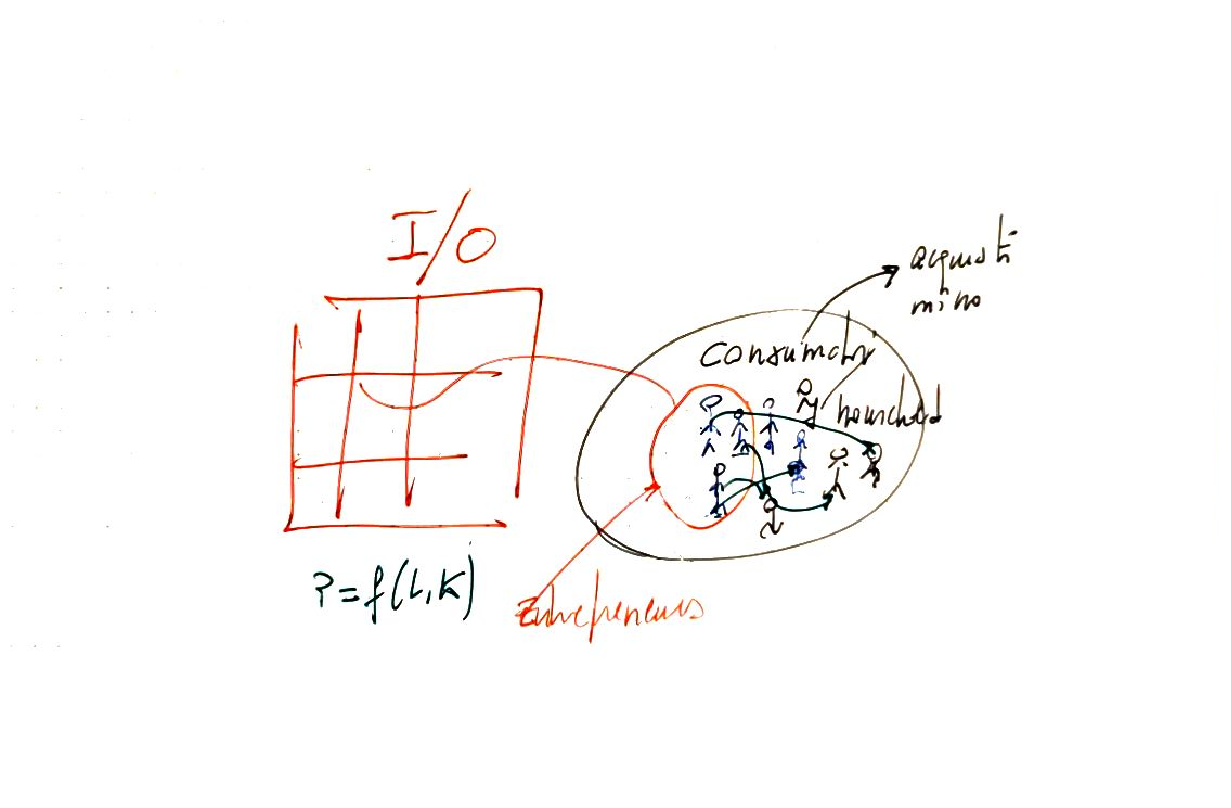
\includegraphics[scale=0.50]{1.pdf}
\label{1}
\caption{Produzione e consumo micro micro}
\end{figure}

\end{frame}

%%%%%%%%%%%%%%%%%%%%%%%%%%%%%%%%%%%%%%%%%%%%%%%%%%%%%%%%%
\begin{frame}{~} % 2



\begin{figure}[H]
\center
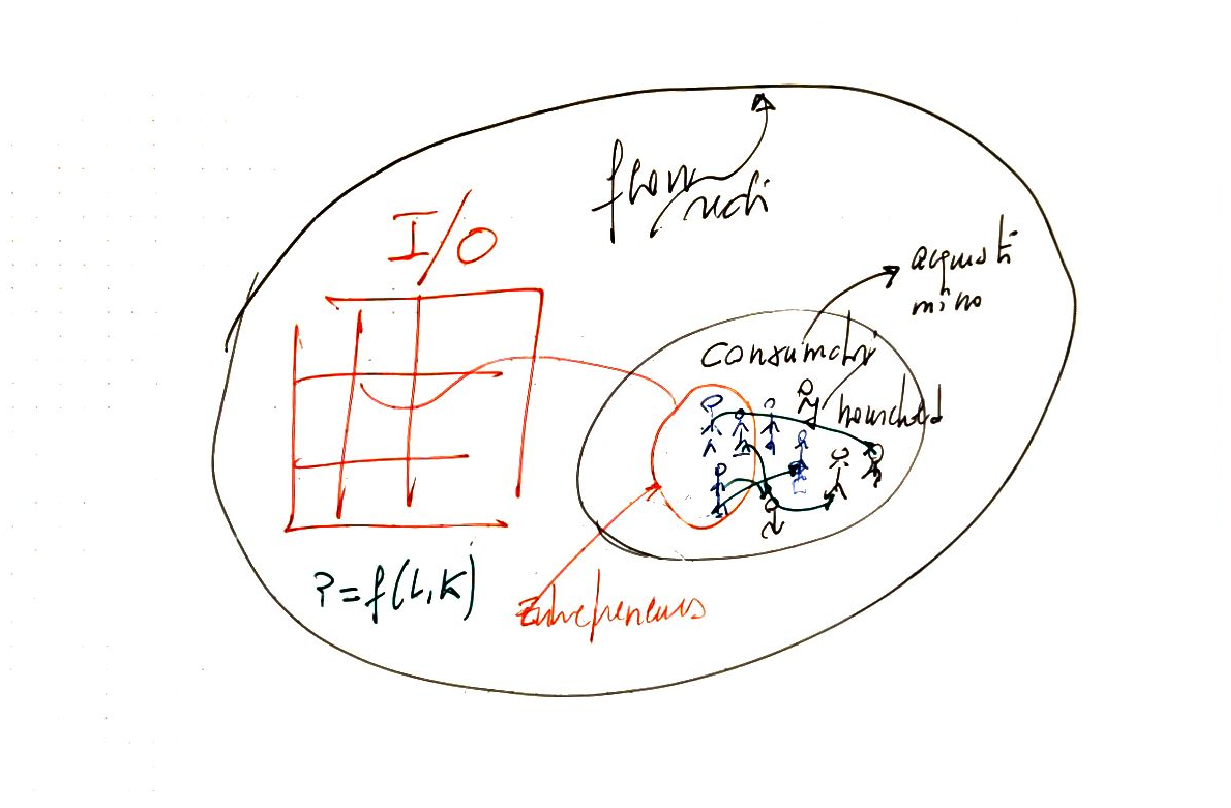
\includegraphics[scale=0.50]{2.pdf}
\label{2}
\caption{Quadratura flussi reali, con produzione, consumi e \ldots}
\end{figure}

\end{frame}

%%%%%%%%%%%%%%%%%%%%%%%%%%%%%%%%%%%%%%%%%%%%%%%%%%%%%%%%%
\begin{frame}{~} % 3



\begin{figure}[H]
\center
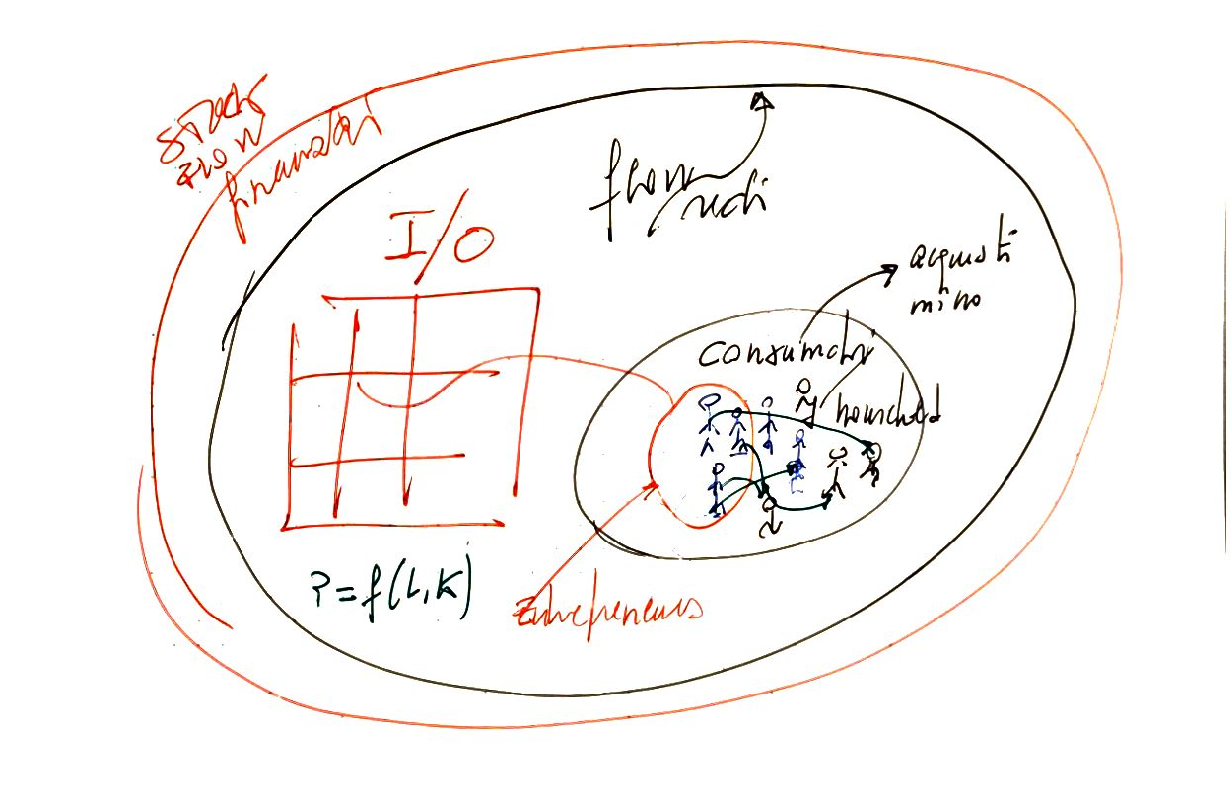
\includegraphics[scale=0.50]{3.pdf}
\label{3}
\caption{Quadratura stock flussi finanziari, con produzione, consumi e \ldots}
\end{figure}

\end{frame}

%%%%%%%%%%%%%%%%%%%%%%%%%%%%%%%%%%%%%%%%%%%%%%%%%%%%%%%%%
\begin{frame}{~} % 4



\begin{figure}[H]
\center
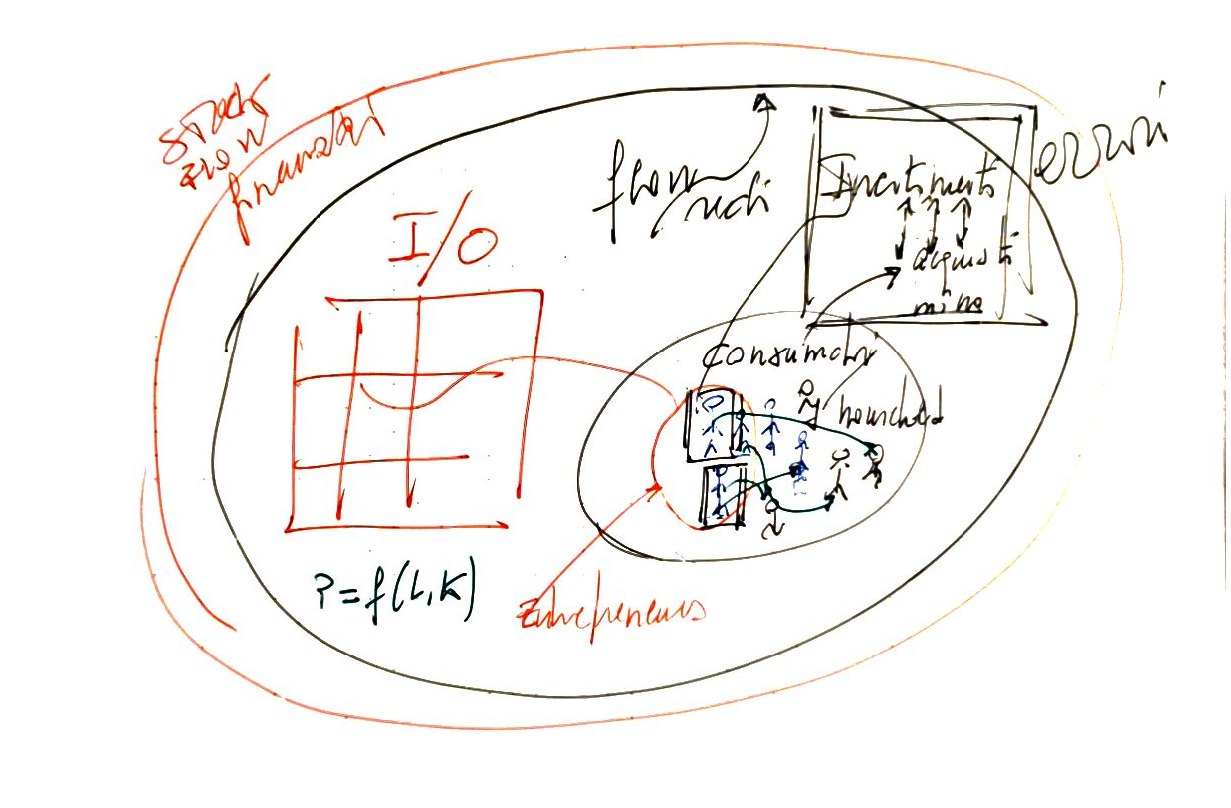
\includegraphics[scale=0.50]{4.pdf}
\label{4}
\caption{\ldots investimenti}
\end{figure}

\end{frame}

%%%%%%%%%%%%%%%%%%%%%%%%%%%%%%%%%%%%%%%%%%%%%%%%%%%%%%%%%
\begin{frame}{~} % 4b



\begin{figure}[H]
\center
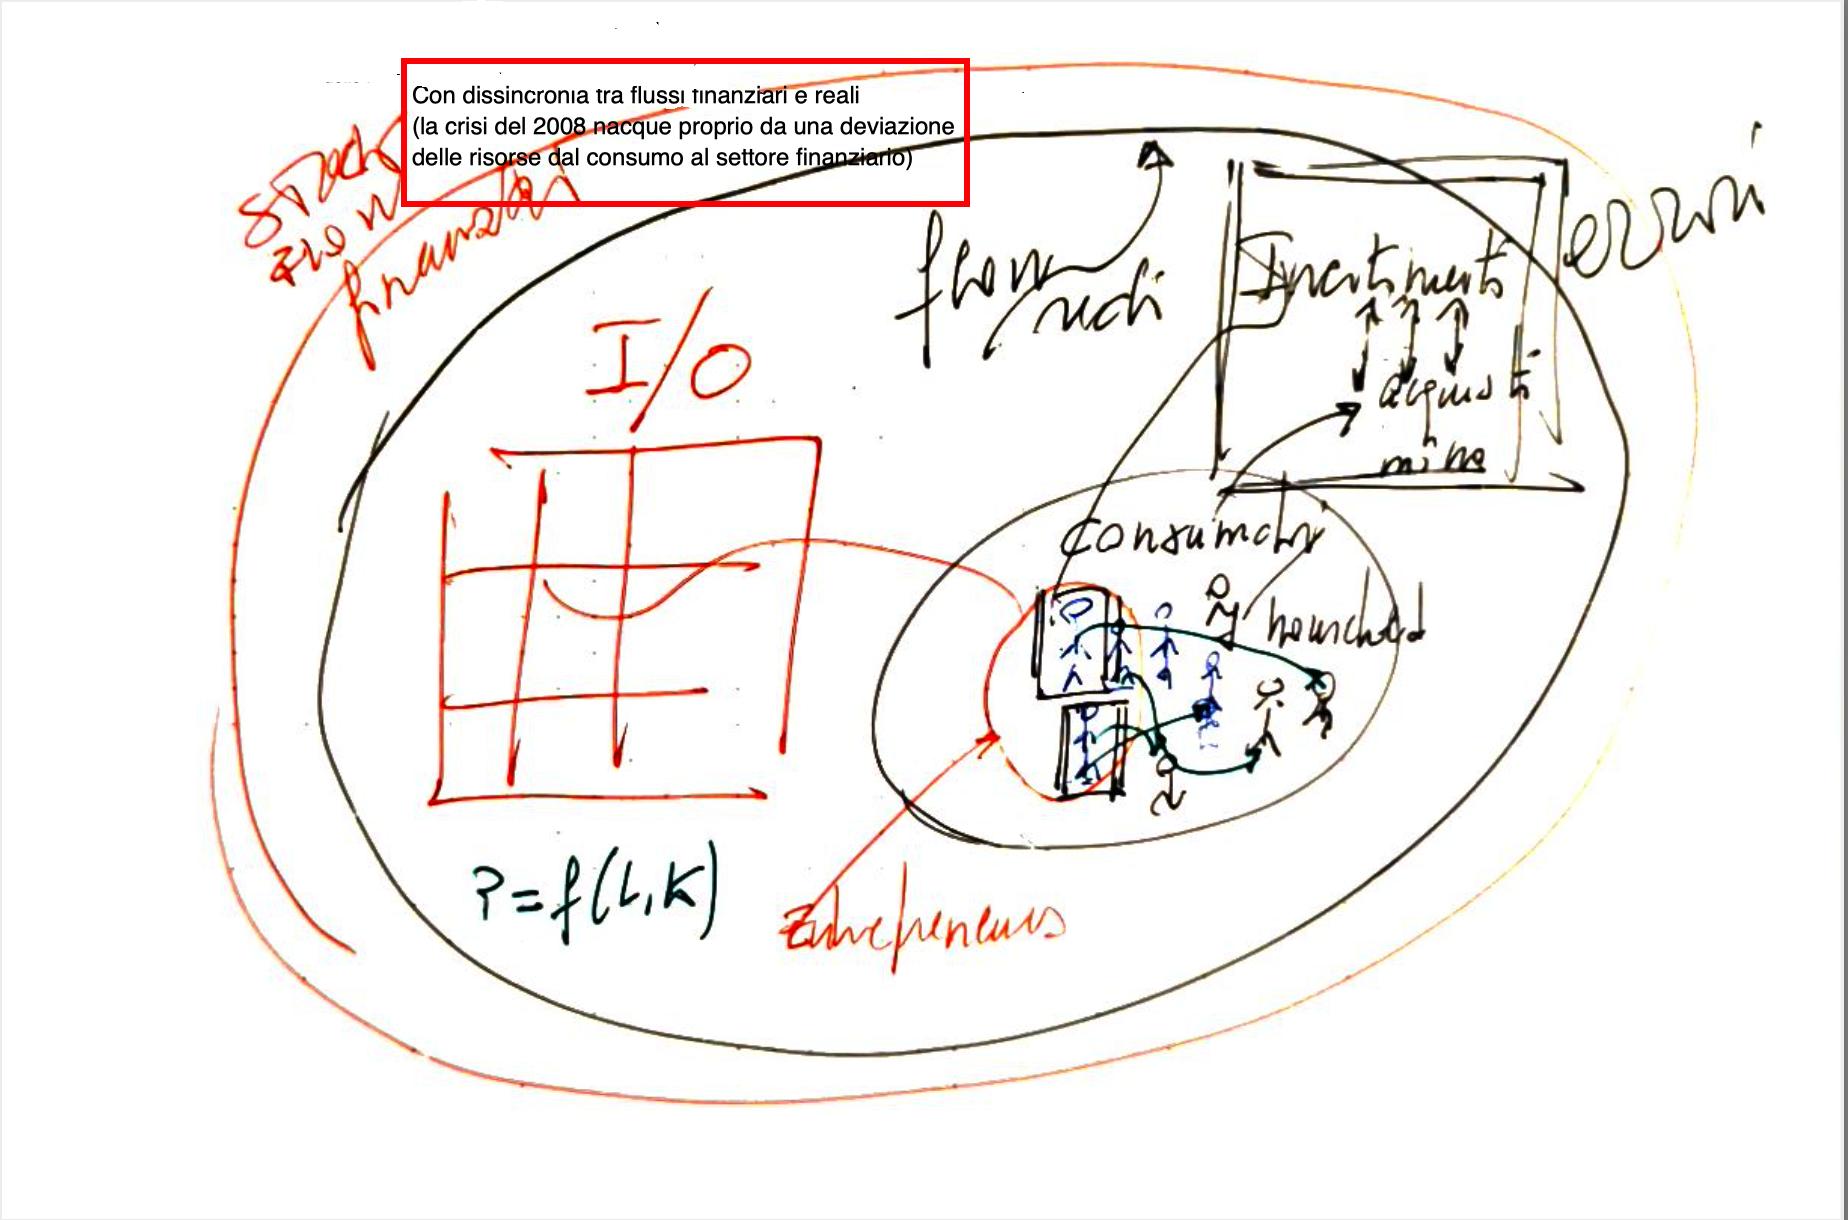
\includegraphics[scale=0.15]{4b.png}
\label{4b}
\caption{\ldots con dirottamente risorse al mondo finanziario}
\end{figure}

\end{frame}

%%%%%%%%%%%%%%%%%%%%%%%%%%%%%%%%%%%%%%%%%%%%%%%%%%%%%%%%%
\begin{frame}{~} % 5



\begin{figure}[H]
\center
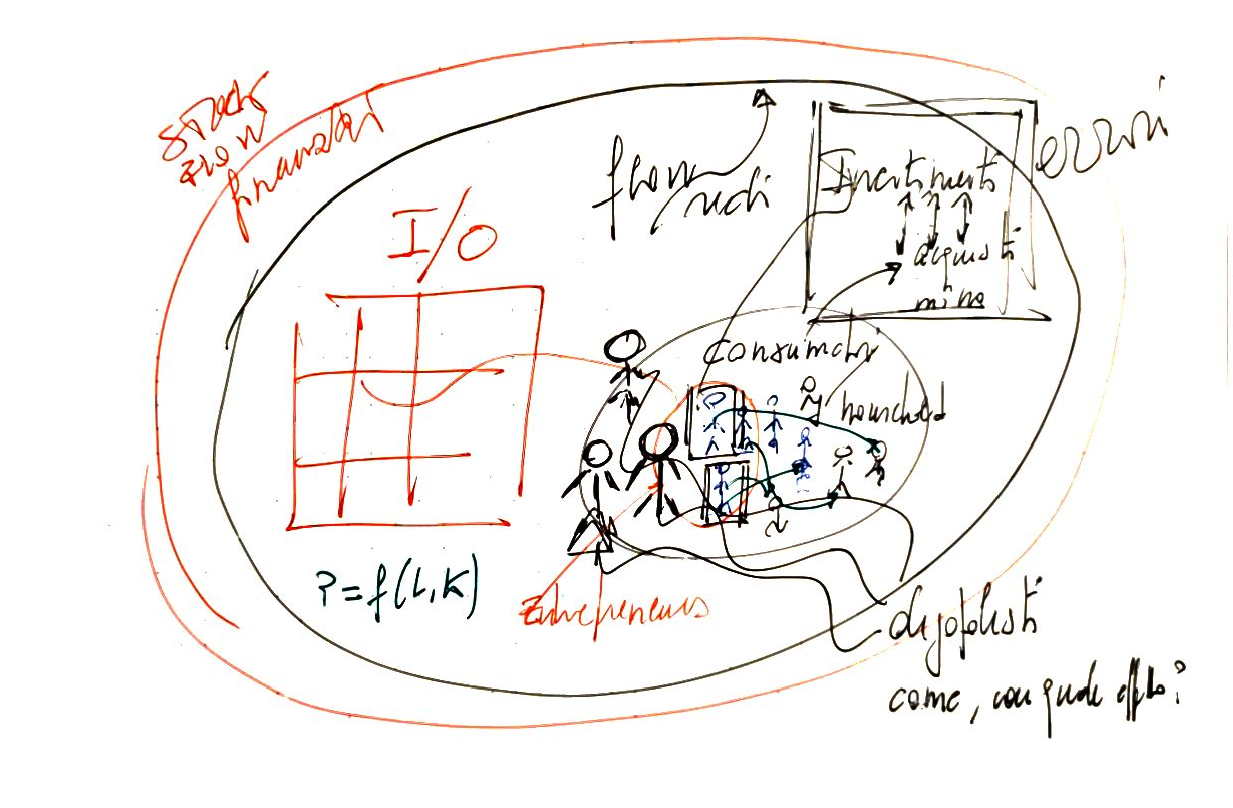
\includegraphics[scale=0.50]{5.pdf}
\label{5}
\caption{Con oligopolisti}
\end{figure}

\end{frame}

%%%%%%%%%%%%%%%%%%%%%%%%%%%%%%%%%%%%%%%%%%%%%%%%%%%%%%%%%
\begin{frame}{~} % 6



\begin{figure}[H]
\center
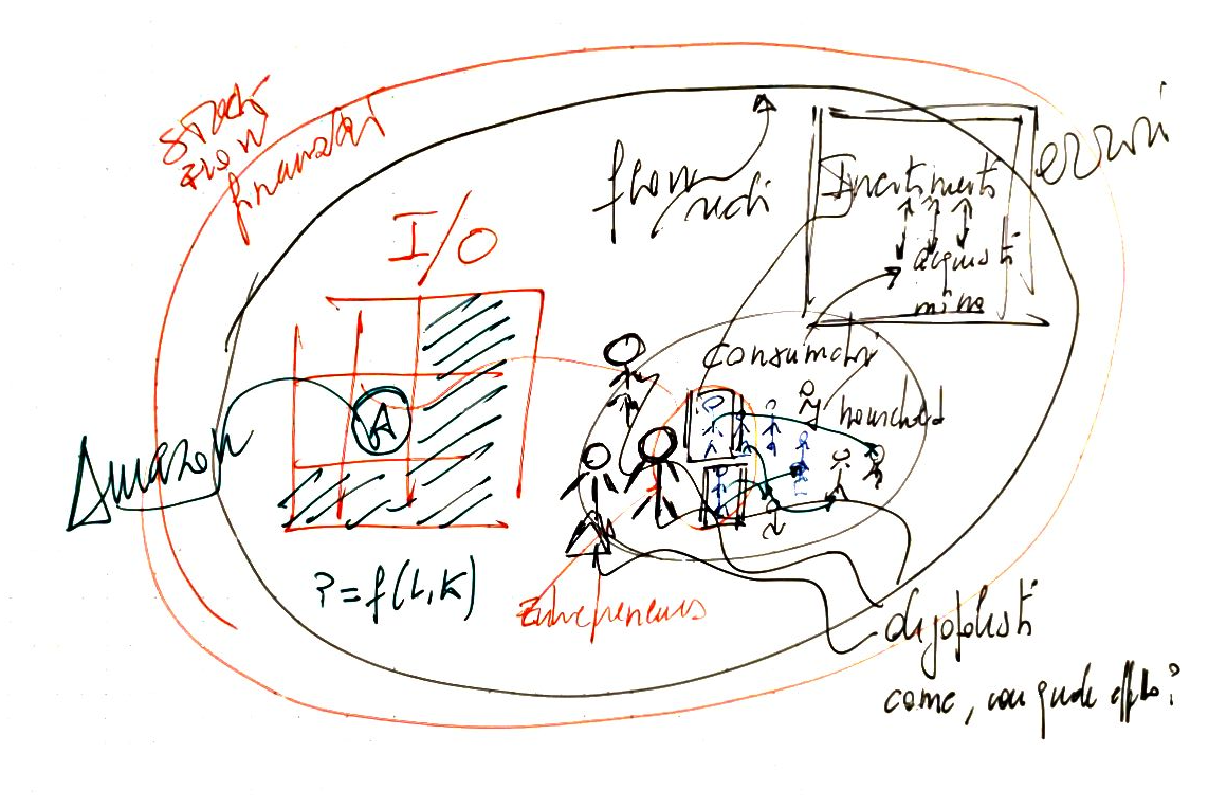
\includegraphics[scale=0.50]{6.pdf}
\caption{Sovrapposizione produzione industriale e commercializzazione e \ldots CHI DECIDE CHE COSA PRODURRE?}
\label{6}
\end{figure}

\end{frame}


%%%%%%%%%%%%%%%%%%%%%%%%%%%%%%%%%%%%%%%%%%%%%%%%%%%%%%%%%
\begin{frame}{~} % 7



\begin{figure}[H]
\center
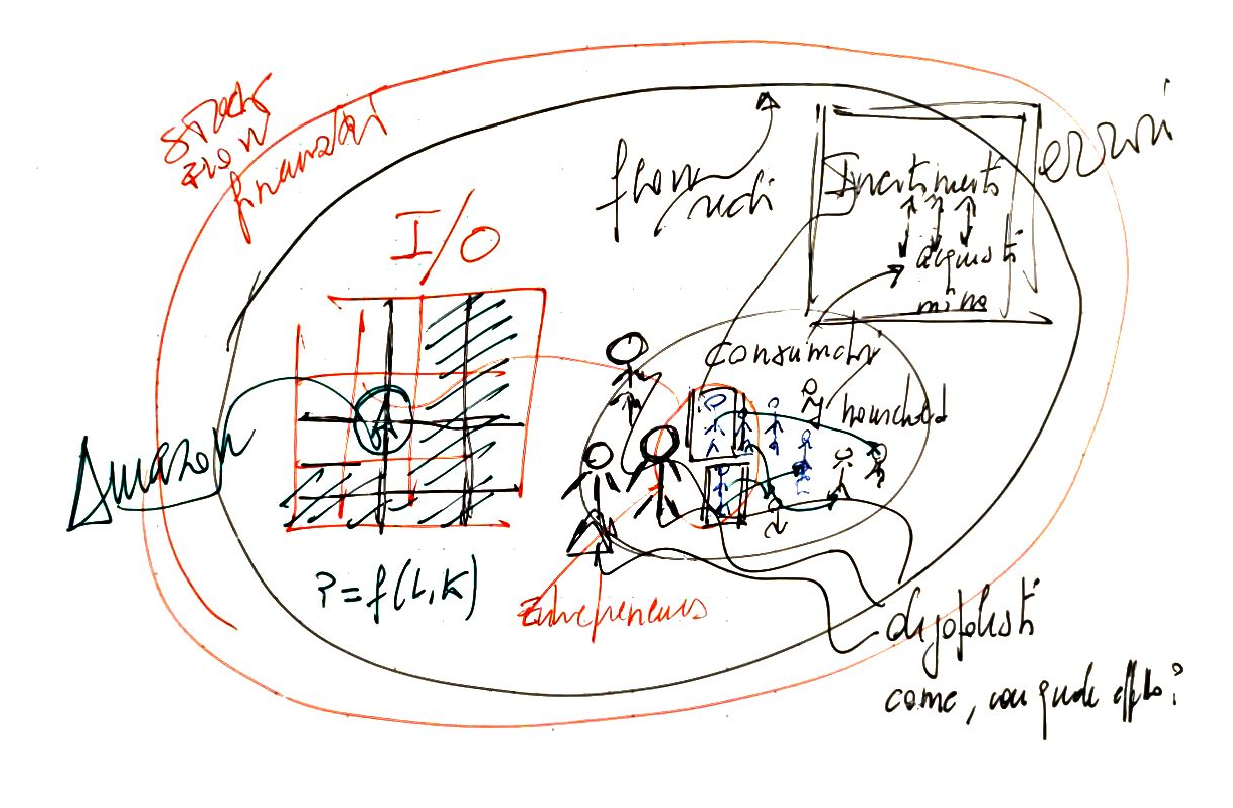
\includegraphics[scale=0.50]{7.pdf}
\label{7}
\caption{Produzione e commercializzazione distinte per beni di consumo e beni investimento}
\end{figure}

\end{frame}

%%%%%%%%%%%%%%%%%%%%%%%%%%%%%%%%%%%%%%%%%%%%%%%%%%%%%%%%%
\section{Linksi}

%%%%%%%%%%%%%%%%%%%%%%%%%%%%%%%%%%%%%%%%%%%%%%%%%%%%%%%%%
\begin{frame}{Queste slide, Overleaf, GitHub, editor formule}

\begin{itemize}

\item
\href{https://terna.to.it/ejmmp/deposito/schemaPietroConLink.pdf}{schemaPietroConLink.pdf}

\item
sta in \href{https://it.overleaf.com/4892961924fddsgrqnbwhh}{Overleaf} con riserva in \href{https://github.com/terna/ejmmpSchemaPietro}{GitHub}

\item
\href{https://editor.codecogs.com}{editor di formule}

\end{itemize}


\end{frame}

%%%%%%%%%%%%%%%%%%%%%%%%%%%%%%%%%%%%%%%%%%%%%%%%%%%%%%%%%
\begin{frame}{Deposito e link}

\href{https://terna.to.it/ejmmp/deposito/}{Deposito}, con:

\begin{itemize}

\item
un \href{https://terna.to.it/ejmmp/deposito/JackIonHayek'sEconomics.pdf}{paper} e una \href{https://terna.to.it/ejmmp/deposito/JackIIonHayek-NoteOnAtomicInvestmentProcesses.pdf}{nota} di Jack;

\item
la \href{https://terna.to.it/ejmmp/deposito/MarcoBookProposalTheoreticalModelBookProposal.pdf}{book proposal} di Marco; la nota di Marco si collega al primo modello, del quale abbiamo anche le \href{https://terna.to.it/oligopolyAgentization.pdf}{slide} di una presentazione (eq. \& ABM) che ho fatto a Agentization;

\item
la \href{https://terna.to.it/ejmmp/deposito/PietroBookProposal.pdf}{folle book proposal} di Pietro, cui si collega un \href{https://www.igss-workshop.org}{convegnone} sulla iGSS con la \href{https://www.youtube.com/watch?v=X7DLFvOhqVo}{presentazione} del modello sul virus; sono visibili anche le \href{https://static1.squarespace.com/static/5e0a8466674f5b6963a2e949/t/60bff462ace45c3d0b9f04cf/1623192677563/terna-slides.pdf}{slide} in cui propongo le mappe di calore e le sequenze dei contagi, forse riusabili i qualche modo;

\item
all'idea di iGGS con Genetic Algorithms collego un micro-modello NetLogo costruito per interagire con gli \emph{ABMgnostics}; \`{e}, anche quello, nel deposito, come \href{https://terna.to.it/ejmmp/deposito/theRace.zip}{zip};

\item
sui GA: segnalo la sezione 7.6 del \href{https://arxiv.org/pdf/2108.08885.pdf}{paperone sul virus} con qualche link, cui aggiungo due siti Wikipedia ben fatti (\href{https://en.wikipedia.org/wiki/Genetic_algorithm}{Genetic Algorithms} e \href{https://en.wikipedia.org/wiki/Holland\%27s\_schema\_theorem}{Holland's schema theorem}) e soprattutto la sezione 1 della \href{https://terna.to.it/tesi/massobrio.pdf}{tesi} di Gerson Massobrio.

\end{itemize}

%\href{}{}
\end{frame}


%%%%%%%%%%%%%%%%%%%%%%%%%%%%%%%%%%%%%%%%%%%%%%%%%%%%%%%%%
\begin{frame}{Materiale che pu\`{o} servirci, anche come ispirazione}

Materiale:

\begin{itemize}

\item
un importante \href{https://terna.to.it/ejmmp/deposito/stockFlow.pdf}{paper} ABM/stock-flow;

\item
J. Doyne Farmer, Simulation conference September 1, 2021, \emph{Simulating the economy
(and the financial system in particular)}, \href{https://www.suomenpankki.fi/globalassets/en/financial-stability/payment-and-settelement-system-simulator/events/2021_01_farmer.pdf}{slide}, con riferimenti all'ambiente;

Jack annnota che la presentazione di Farmer sull'ecologia economico utilizza immagini ad una pluralit\`{a} di livelli per modellare una certa realt\`{a}. 
\href{https://en.wikipedia.org/wiki/William_C._Wimsatt}{Wimsatt} negli anni `70 faceva gi\`{a} una cosa simile per far vedere i vari livelli di analisi che si possono applicare ad una certa realt\`{a}. [\emph{Levels of organization in biology}, su Research gate ci sono articoli suoi con questo titolo].

\item 
Mordecai Kurz, \href{http://sfi-edu.s3.amazonaws.com/sfi-edu/production/uploads/sfi-com/dev/uploads/filer/9f/28/9f288132-c3b3-410a-8ff7-2b8303014790/91-02-013.pdf}{On the Structure and Diversity of Rational Beliefs}.



\end{itemize}

%\href{}{}
\end{frame}


%%%%%%%%%%%%%%%%%%%%%%%%%%%%%%%%%%%%%%%%%%%%%%%%%%%%%%%%%
\section{Note di sintesi}

%%%%%%%%%%%%%%%%%%%%%%%%%%%%%%%%%%%%%%%%%%%%%%%%%%%%%%%%%
\begin{frame}{Memo di Eleonora sulla giornata}

\scriptsize


\begin{itemize}

\item
Il progetto (assai ambizioso) \`{e} quello di scrivere la \emph{storia del futuro della macroeconomia}, simulando le nuove dinamiche emergenti che la caratterizzano.

\item
La baseline \`{e} quella di uno scenario dove tutti gli agenti sono consumatori e alcuni di essi sono anche produttori con funzione di produzione $P=f(L,K)$, con l'obiettivo pratico di modellizzare agente per agente un mercato dove gli acquisti (o meglio i tentativi di acquisto) avvengono giorno per giorno e l'obiettivo teorico di dar vita a un modello macroeconomico fondato sui comportamenti micro.

\item
Al centro di questo schema metteremo la \textbf{quadratura dei flussi reali} (fondati su produzione e consumi --- a cui andremo ad aggiungere anche gli \textbf{investimenti}) con gli \textbf{stock e i flow finanziari}. \`{a} cruciale osservare in tutto questo il ruolo degli investimenti, dal momento che saranno gli errori negli investimenti (intesi nei termini della teoria delle aspettative, ma anche e soprattutto come conflitto tra i diversi agenti derivante anche da una contraddizione tra sistemi informativi --- che a sua volta dipende dalle reti di collegamento e che rimanda alla teoria dei rational beliefs di Mordecai Kurz) a dar luogo agli \textbf{shock economici}. Da qui lo spunto di utilizzare la \textbf{teoria dei cicli economici hayekiana} per spiegare le \textbf{crisi} (in primis quella del 2008, ma soprattutto quelle a venire): fenomeni che possiamo leggere nei termini di dissincronia tra flussi finanziari e reali (del resto la crisi del 2008 nacque proprio da una deviazione delle risorse dal consumo al settore finanziario).

\item
A questo punto, se facciamo le cose bene, mettendo a sistema il \textbf{rapporto tra produzione, commercio e pianificazione} il nostro modello dovrebbe essere in grado di mostrarci \textbf{quali macro-strutture di mercato possono emergere} (e.g. oligopoli e superoligopoli \'{a} la Amazon).

\item
Come indicato nelle slide, sezione strumenti e anche book proposal di Pietro, l'idea \`{e} quella di passare da un tradizionale modello ad agenti con propriet\`{a} emergenti ``pianificate'' a livelli di complessit\`{a} pi\`{u} alti in cui gli agenti attingono a dei menu di scelta per definire i loro comportamenti, e attraverso algoritmi genetici, generare nuovi items all'interno di questi menu di scelta, con l'obiettivo di inserirci nella cornice teorica della cd \emph{inverse generative social science} che, a partire da una fotografia della società ci consente attraverso le simulazioni di trovare possibili spiegazioni dei meccanismi che danno luogo a questa.

\item
Per quanto riguarda la lettura dei risultati, il lavoro ``viruloso'' di Pietro offre due preziosi spunti. Uno, fare tante simulazioni per osservare la distribuzione delle frequenze dei risultati, utilizzando magari  delle simpatiche mappe di calore (per esempio per osservare i casi dei cd \emph{too big to fail}); due, guardare alle storie individuali degli agenti in una singola simulazione per osservare quali condizioni generano quali scenari (molto interessante eg per studiare il ruolo delle policies).

\end{itemize}

\end{frame}


%%%%%%%%%%%%%%%%%%%%%%%%%%%%%%%%%%%%%%%%%%%%%%%%%%%%%%%%%
\begin{frame}{Addendum di Jack (1/2)}

\scriptsize

\begin{itemize}

\item
Per analizzare la crisi del 2007 e quella prossima (ho appena comprato The Economist al prezzo scandaloso di 8,50 euro) in termini hayekiani ovvero come deviazione di risorse da investimenti/prodotti ``utili'' nel settore reale a investimenti nel settore finanziario \textbf{oltre il limite della funzione di ausiliari per il funzionamento dei mercati finanziari} dobbiamo trattare prodotti derivati (anche al quadrato e alla terza potenza ovvero derivati di derivati ecc.) nello stesso modo/allo stesso livello. Questa importante apertura del modello comporta la soluzione di questo problema.

\item
In questa prospettiva potremmo magari trasformare un problema fondamentale di modelli di equilibrio intertemporale in un'opportunit\`{a}. Il problema \`{e} la definizione di un bene: fragole ad agosto non sono lo stesso bene di fragole a gennaio. Conseguenza: l'esplosione del numero dei beni e quindi dei mercati, cosa che diventa ingestibile. Dalla rivoluzione marginale non possiamo pi\`{u} ammettere la definizione di un bene in termini fisici: quello che \`{e} un bene dipende dalla percezione degli individui: un bene \`{e} quello che soddisfa certe determinate esigenze/preferenze soggettive. Portata alla sua conclusione logica significherebbe che possono esserci tanti beni quanti individui. Ci salva (almeno un po') l'esistenza dei mercati. Gli individui che entrano in un rapporto di scambio di A devono necessariamente avere una percezione congruente di quello che costituisce A. Potrebbe essere l'inizio della soluzione del problema della definizione di un bene?


\end{itemize}

\end{frame}

%%%%%%%%%%%%%%%%%%%%%%%%%%%%%%%%%%%%%%%%%%%%%%%%%%%%%%%%%
\begin{frame}{Addendum di Jack (2/2)}

\scriptsize

\begin{itemize}

\item
L'esistenza di economie centralmente pianificate come Amazon all'interno di un'economia di mercato ci porta a rispolverare il ``debate on socialism'' degli anni '30. Ora, come scrive Hayek (credo in Economics and knowledge, "non \`{e} se si pianifica o meno ma chi pianifica [effettivamente, bisogna aggiungere]: tutti gli individui oppure Bezos. In altre parole, quello che conta \`{e} il livello di pianificazione effettiva (per cui intendo la pianificazione che ha delle conseguenze a livello macro). Tradotto in termini di coordinazione: in Bezosland si pu\`{o} porre la domanda chi coordina ma in un'economia decentralizzata, dove nessuno coordina, la domanda diventa: che cosa coordina i comportamenti individuali. Risposta il mercato e il sistema dei prezzi.

Dobbiamo eliminare il concetto dell'inflazione dal nostro modello. Gli individui non percepiscono l'inflazione (tranne sulle pagine della stampa, un'esempio del successo di una certa scuola di pensiero economico che ha fatto un lavaggio dei cervelli in modo che un concetto metafisico \`{e} diventato parte della realt\`{a} studiata dalla stessa teoria economica) ma solo dei prezzi specifici. A me da senza tetto non importa niente se il tasso d'inflazione \`{e} salito a seguito dei costi dell'abitazione (una grossa percentuale del paniere Istat) perch\'{e} non abito. Sia Pietro sia Marco hanno rilevato l'importanza della comunicazione e qui ci aspetta un compito difficile nei confronti dei nostri colleghi economisti. Persino nella stampa informata quale il Financial Times la causalit\`{a} sembra invertita: \`{e} facile trovare espressioni come``l'inflazione ha portato all'aumento del prezzo della case'' (avevo salvato degli esempi ma li cercher\`{o} con calma). No! \`{E} l'aumento dei prezzi immobiliari che ha fatto salire la statistica che chiamiamo inflazione. Abbasso l'essenzialismo in economia!


\item
Il contagio come modellato nella presentazione di Pietro del suo modello AB applicato al covid: mi sembra eminentemente applicabile al fenomeno del too important to fail, dove important = totale di bilancio di un'istituzione finanziaria + il numero e il peso della connessioni con altre istituzioni finanziarie. Meno facile da modellare ma concettualmente possibile mi sembra un'estensione al settore reale, per esempio supply chain problems: la non disponibilit\`{a} di chips rallenta o blocca la produzione delle automobili. Altro esempio: il fallimento di Stellantis avrebbe degli effetti devastanti sull'indotto.

\end{itemize}

\end{frame}

%%%%%%%%%%%%%%%%%%%%%%%%%%%%%%%%%%%%%%%%%%%%%%%%%%%%%%%%%
\section{Strumento e primi passi}

%%%%%%%%%%%%%%%%%%%%%%%%%%%%%%%%%%%%%%%%%%%%%%%%%%%%%%%%%
\begin{frame}{Strumenti}

Che cosa usiamo?

\begin{itemize}

\item
\href{https://terna.github.io/SLAPP/}{SLAPP} oppure \ldots

\item
\href{https://repast.github.io/repast4py.site/index.html}{Repast4Py}?

A giugno, un seminario presso IRES Piemonte su Repast4Py (idea di un modello ABM sul Piemonte, microfondato, stock-flow)

\end{itemize}

Portare in giro lavori preliminari?

\href{https://ssc2022.behavelab.org}{SSC2022} is the 17th annual Social Simulation Conference and will take place from 12--16 September 2022 at the University of Milan, Italy.

\href{https://ssc2022.behavelab.org/submissions/}{Deadline} 15 May 2022.

%\href{}{}
\end{frame}

\end{document}

